\documentclass[svgnames]{beamer}

\usepackage{pri}
\usepackage{pstricks}
\usepackage{pst-tree}
\usepackage{pst-node}
\usepackage{colortbl}
\usepackage{comment}

\SpecialCoor                  % para usar nodes como coordenadas (pstricks)


% as figuras podem estar numa destas pastas:
\graphicspath{{./}{figures/}{figures/02-intro-IR/}}


\title{Processamento e Recuperação de Informação}

\subtitle{Introduction to Information Retrieval}

\begin{document}

\maketitle
\makeoutline

\section{Scope of IR topics}

\begin{frame} \frametitle{Concepts to be Covered}

\begin{itemize}
   \item Basic Concepts of Information Retrieval (IR)
   \item Classic Information Retrieval Models

   \item Advanced Information Retrieval Models (BM25, $N$-Gram Language Models, ...)
   
   \item Different Types of IR Tasks

   \item IR Evaluation

   \item Inverted Indexes and Query Processing

   \item Web Search and Advanced Search Results Ranking

   \item Meta-search
\end{itemize}

\end{frame}


\begin{frame} \frametitle{Bibliography}

    \begin{block}{}
      \href{http://www.mir2ed.org/}{Ricardo Baeza-Yates,
            Berthier Ribeiro-Neto, Modern Information Retrieval, 2nd
            edtion}. \href{http://grupoweb.upf.es/WRG/mir2ed/pdf/chapter1.pdf}
          {Chapter 1 \emph{(download)}}, and beginning of Chapter 3.
    \end{block}

    \begin{block}{}
      \href{http://www.cs.uic.edu/~liub/WebMiningBook.html}{Bing Liu, Web Data Mining: Exploring Hyperlinks, Contents, and Usage Data, 2nd edition}. Chapter 6.   
    \end{block}

    \begin{block}{}
      \href{http://nlp.stanford.edu/IR-book/}{Christopher D. Manning, Prabhakar Raghavan and Hinrich Schütze, Introduction to Information Retrieval}. Beginning of Chapters 1, 2, 6 and 19 (\href{http://nlp.stanford.edu/IR-book/}{\emph{all online}}). 
    \end{block}

\end{frame}

%----------------

\begin{frame}
  \frametitle{Information Retrieval}

\begin{block}{}

IR deals with the representation, storage, organization of, and
  access to information items of various types:

\begin{itemize} 
    \item documents, 
    \item Web pages,
    \item online catalogs, 
    \item structured records,
    \item multimedia objects,
    \item ...
\end{itemize}

\end{block}

\end{frame}


\begin{frame}
  \frametitle{Information Retrieval: Goals}

  \begin{columns}[t]

    \column{0.4\textwidth}

    \begin{block}{Early goals in IR:} indexing text and
      searching for useful documents in a collection. 
    \end{block}

    \column{0.4\textwidth}

    \begin{block}{Current research goals:}
      \begin{itemize} 
      \item Modeling, 
      \item Web search,
      \item text classification, 
      \item systems architecture, 
      \item user interfaces, data visualization, 
      \item filtering and
      \item human language technologies (e.g., in dialogue systems).
     \end{itemize}
\end{block}

\end{columns}

\end{frame}


\begin{frame}
  \frametitle{IR at the Centre of the Stage}

\begin{block}{}
Until recently, IR was an area of interest restricted mainly to
librarians and information experts. 
\end{block}

\begin{block}{}
A single fact changed these perceptions -- the introduction of the
\textbf{Web}, the largest repository of knowledge in human history. 

Due to its enormous size, finding useful information on the Web
usually requires \alert{running a search} 
\end{block}


\begin{block}{$\Rightarrow$ Searching on the Web is all about IR and its technologies}
\end{block}



\end{frame}

% ------------------------------------------------------------


\section{The IR Problem}


\begin{frame}
\frametitle{The IR Problem}
Ad-hoc retrieval is perhaps the core problem
\vfill
Users of modern IR systems, such as search engine users, have information needs of varying complexity

\begin{block}{An example of complex information need is as follows:}
{\it Find all documents that address the role
of the Federal Government in financing
the operation of the National Railroad
Transportation Corporation (AMTRAK)}
\end{block}

\end{frame}



\begin{frame}
  \frametitle{The IR Problem}

\begin{itemize}

\item This full description of the user information need is not necessarily a good query to be submitted to the IR system
\item Instead, the user might want to first translate this information need into a \alert{query}
\item This translation process yields a set of keywords, or index terms, which summarize the user information need
\end{itemize}

\vfill

\begin{block}{}
Given the user query, the key goal of the IR system is to retrieve
information that is useful or relevant to the user
\end{block}

\end{frame}



\begin{frame}
  \frametitle{The IR Problem: Relevance}

\begin{block}{}
 The IR system must \alert {rank the information items} according to a degree of \alert{relevance} to the user query
\end{block}

\begin{block}{The IR Problem}
The key goal of an IR system is to retrieve all the items that are relevant to a user query, while retrieving as few nonrelevant items as possible
\end{block}

\begin{block}{}
 The vague notion of \alert{relevance is of central importance in IR}
\end{block}

\end{frame}

\begin{frame}
  \frametitle{The User's Task}

\begin{block}{Consider a user who seeks information on a topic of interest}

\begin{itemize}

\item This user first translates his/her information need (e.g., find the author of a book) into a query

\begin{itemize} \item requires specifying the words that compose the
  query 
\end{itemize}

\item In this case, we say that the user is \alert{searching} or \alert{querying} for
information of his/her interest

\end{itemize}
\end{block}

\begin{block} {Consider now a user who has an interest that is either poorly defined or inherently broad}
\begin{itemize}
 \item For instance, the user has an interest in car racing and wants to browse documents on Formula 1 and Formula Indy
\item In this case, we say that the user is \alert{browsing} or \alert{navigating} the documents of the collection
\end{itemize}
\end{block}

\end{frame}

\begin{frame}
\frametitle{The User's Task}

\begin{center}
  \includegraphics[width=0.8\textwidth]{user-interaction.png}
\end{center}

\end{frame}

\begin{frame}
  \frametitle{Information vs. Data Retrieval}

  \begin{block}{Data retrieval}
    Given a specified condition (e.g.~$\{\text{lab}, \text{ethics}\} \in
    \text{document}$), find all items that satisfy the condition
  \end{block}

  \begin{center}
    {\Huge $\neq$}
  \end{center}

  \begin{block}{Information retrieval}
    Given a user query, find all items that contain information
    \emph{relevant} to the user's needs
  \end{block}

  \pause

  \begin{block}{However...}
    ... how do you characterize the \alert{user's information need}?
  \end{block}


\end{frame}

% ------------------------------------------------------------

\begin{frame} \frametitle{Translating the user information need}
  
  \begin{block}{An example}
    \begin{quote}
      Find all Web pages containing information on the ethical treatment of
      animals for medical experiments. The pages should contain references to
      recent related scientific articles, together with an enumeration of known
      existing alternatives for different medical fields.
    \end{quote}
    \begin{flushright}
      \small
      \href{http://www.google.pt/search?q=Find+all+Web+pages+containing+information+on+the+ethical+treatment+of\%0D\%0A++++++animals+for+medical+experiments.+The+pages+should+contain+references+to\%0D\%0A++++++recent+related+scientific+articles\%2C+together+with+an+enumeration+of+known\%0D\%0A++++++existing+alternatives+for+different+medical+fields.}{\alert{try this on Google}}
    \end{flushright}
  \end{block}

  \pause

  \begin{block}{}
    Usually this is translated to
    \begin{center}
      \href{http://www.google.pt/search?q=ethics+animals+medical+experiments}{ethics animals medical experiments}
    \end{center}
    \vspace{-1\baselineskip}
    \begin{flushright}
      but is this a convenient translation?
    \end{flushright}
  \end{block}


\end{frame}

% ------------------------------------------------------------

% ------------------------------------------------------------

\section{IR Systems}


\begin{frame}
  \frametitle{IR Tasks}

  \begin{columns}[t]

    \column{0.4\textwidth}

    \begin{block}{Document processing}
      \begin{itemize}
      \item Crawling
      \item Segmenting and annotating
      \item Indexing
      \item Query processing
      \item Distributed IR
      \item String processing
      \item ...
      \end{itemize}
    \end{block}

    \column{0.4\textwidth}

    \begin{block}{Information processing}
      \begin{itemize}
      \item \emph{\href{http://www.google.com}{\textit{Ad-hoc} retrieval}}
      \item \href{http://www.dmoz.org/}{Classification}
      \item \href{http://vivisimo.com/}{Clustering}
      \item \href{http://www.last.fm/}{Filtering}
      \item \href{http://textsummarization.net}{Summarization}
      \item \href{http://www.ibm.com/watson/}{Question answering}
      \item ...
      \end{itemize}
    \end{block}

  \end{columns}
\end{frame}

% ------------------------------------------------------------

\begin{comment} %% next slide is better

\begin{frame}
  \frametitle{The Retrieval Process}

  \begin{block}{}
    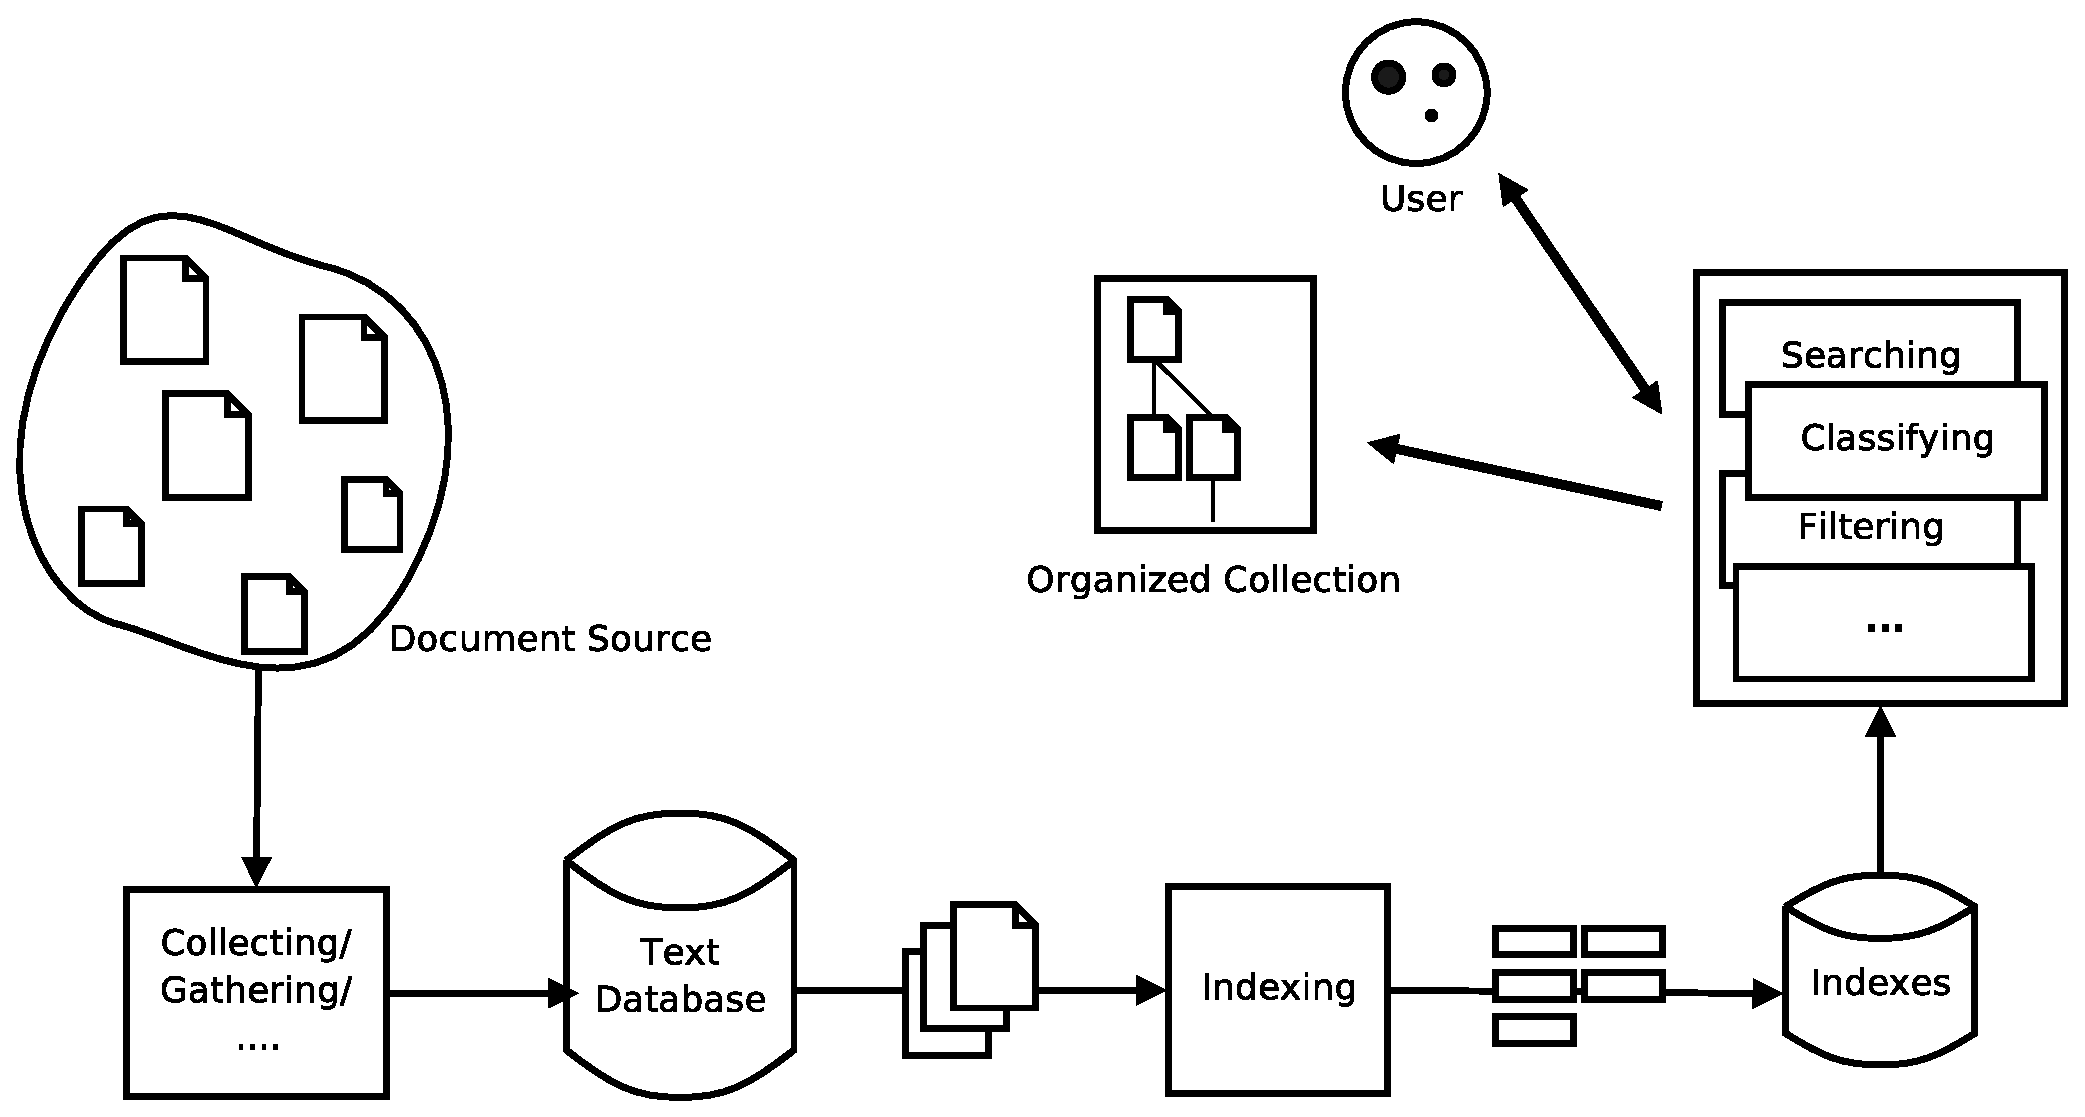
\includegraphics[width=\textwidth]{process}
  \end{block}
\end{frame}

\end{comment}



\begin{frame}
 \frametitle{The Retrieval Process}

 \begin{block}{}
     \includegraphics[width=0.8 \textwidth]{process-mir2ed}
  \end{block}
\end{frame}


\begin{comment} %% too complex for EADW, not shown.

\begin{frame}
  \frametitle{The Retrieval Process}

  \begin{block}{}
    \includegraphics[width=0.7 \textwidth]{process-mir2ed-2nd}
  \end{block}
\end{frame}

\end{comment}



%\newcommand{\Mnode}[2][]{\TR{\psframebox[fillstyle=solid,#1]{\textcolor{white}{#2}}}}

\begin{frame}
   \frametitle{A First Proposal: Memex}
  
  \begin{center}
    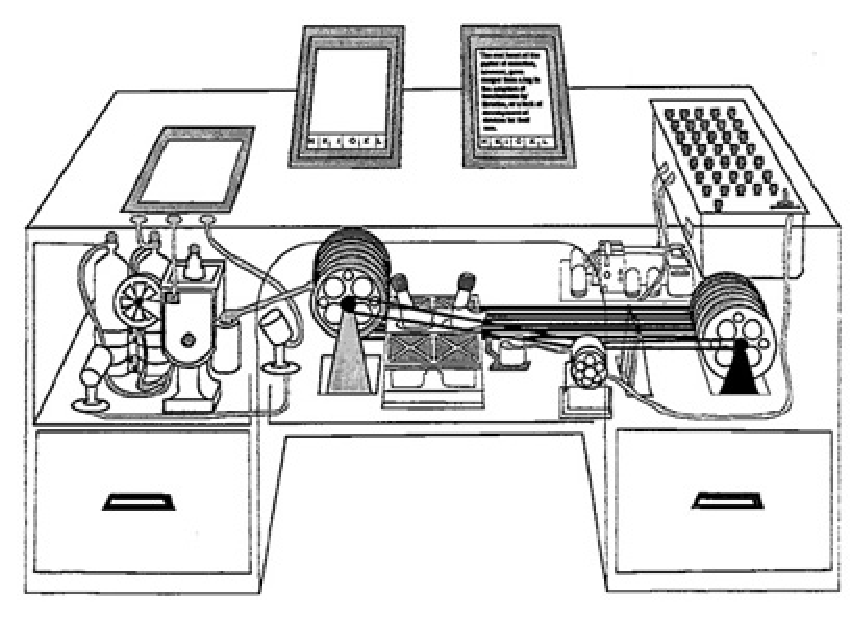
\includegraphics[width=.8\linewidth]{memex}\\
    \raggedleft \footnotesize Bush, V. \textit{As We May Think}, 1945
  \end{center}

\end{frame}

% ----------------------------------------------------------------------

\begin{frame}
  \frametitle{A First Solution: Universal Card Scanner }

  \begin{center}
    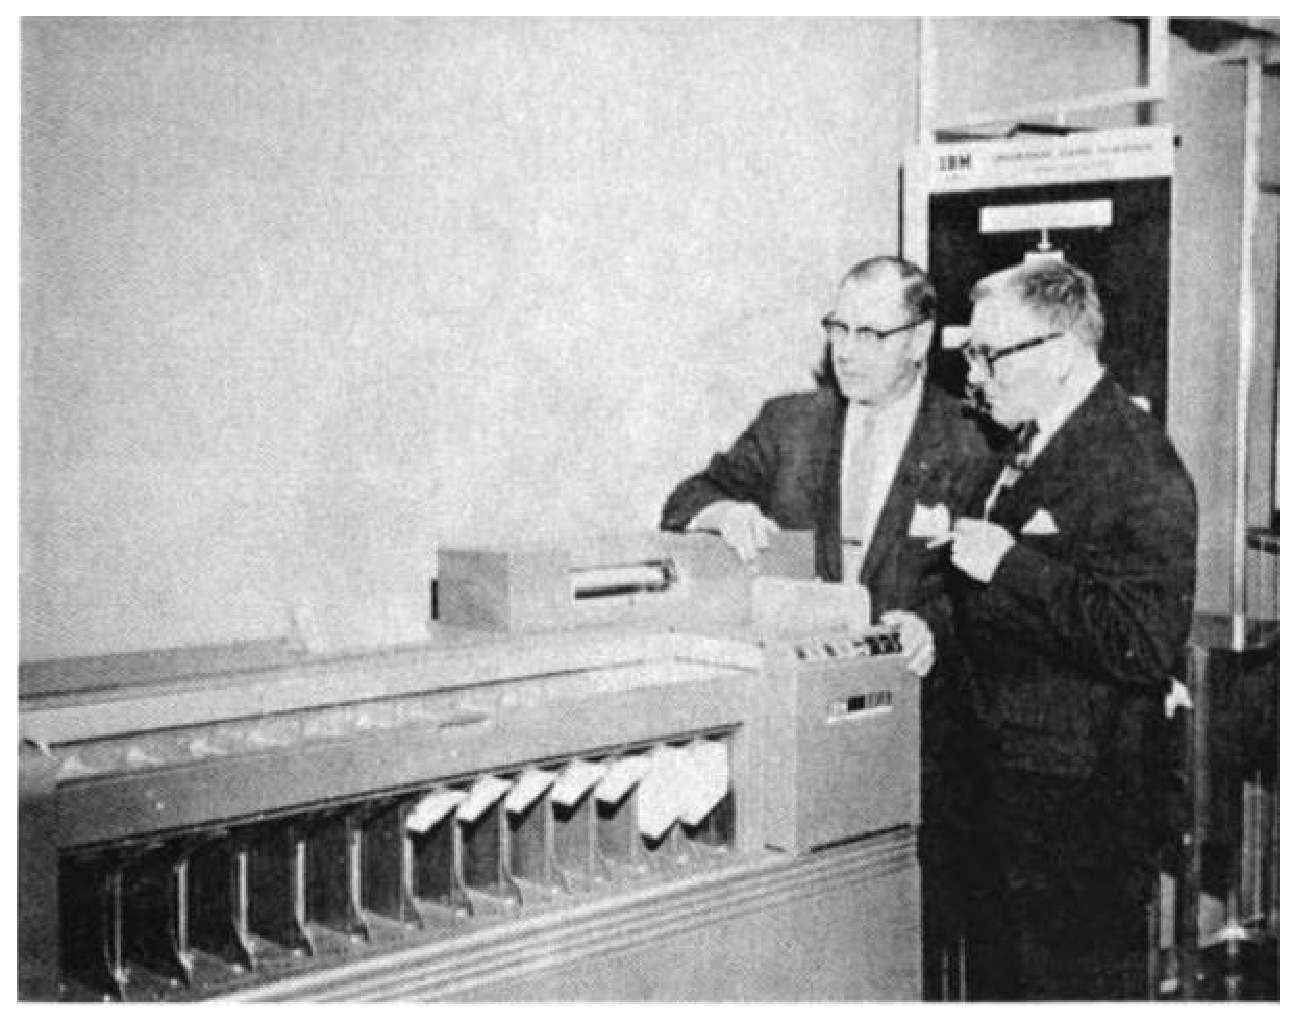
\includegraphics[width=.8\linewidth]{luhn}\\
    \raggedleft \footnotesize Luhn, H. P. 1950(--1958)
  \end{center}

\end{frame}

% ------------------------------------------------------------

\section{Modeling}
\label{sec:modeling}

\newcommand{\ff}[1]{\visible<3-4>{\textcolor{Red}{#1}}}
\newcommand{\sw}[1]{\uncover<-3>{#1}}
%\newcommand{\pl}{\cline{1-4}\cline{6-8}}
\newcommand{\pl}{\hline\hline}
\newcommand{\vl}{\hfill\vline}

\begin{frame}
  \frametitle{Models for Information Retrieval}

  \begin{center}
    \includegraphics[width=.5\linewidth]{bag-of-words-sculpture}\\
    \raggedleft \footnotesize Art installation of a bag of words @ CMU  
  \end{center}
\end{frame}

\begin{frame}
  \frametitle{An Example}

  \only<1>{
    \begin{block}{Example document}
      \begin{quote}
        I heartily accept the motto, ``That government is best which governs
        least''; and I should like to see it acted up to more rapidly and
        systematically. Carried out, it finally amounts to this, which also I
        believe---``That government is best which governs not at all''; and
        when men are prepared for it, that will be the kind of government which
        they will have.
      \end{quote}
    \end{block}
  }

  \only<2-4>{
    \begin{block}{Index terms}
      \small
      \begin{tabular}{|c@{\hspace{0.09mm}}|@{\hspace{0.09mm}}c@{\hspace{0.09mm}}|@{\hspace{0.09mm}}c@{\hspace{0.09mm}}|@{\hspace{0.09mm}}c@{\hspace{0.09mm}}|@{\hspace{0.09mm}}c@{\hspace{0.09mm}}|@{\hspace{0.09mm}}c|} \hline
        \sw{I \ff{3}} & accept \ff{1} & acted \ff{2} & all \ff{3} & \sw{also \ff{1}} & amounts \ff{1} \\\hline

        \sw{and \ff{3}} & are \ff{1} & \sw{at \ff{1}} & be \ff{1} & believe \ff{1} & best \ff{2} \\\hline

        carried \ff{1} & finally \ff{1} & \sw{for \ff{1}} & government \ff{3} & governs \ff{2} & have \ff{1} \\\hline

        heartily \ff{1} & is \ff{2} & \sw{it \ff{3}} & kind \ff{1} & least \ff{1} & like \ff{1} \\\hline

        men \ff{1} & more \ff{1} & motto \ff{1} & \sw{not \ff{1}} & \sw{of \ff{1}} & out \ff{1} \\\hline

        prepared \ff{1} & rapidly \ff{1} & see \ff{1} & should \ff{1} & systematically \ff{1} & \sw{that \ff{3}} \\\hline

        \sw{the \ff{2}} & \sw{they \ff{1}} & \sw{this \ff{1}} & \sw{to \ff{3}} & \sw{up \ff{1}} & \sw{when \ff{1}} \\\hline
 
        \sw{which \ff{4}} & will \ff{2} & & & & \\\hline
      \end{tabular}
    \end{block}
  }

  \only<5->{
    \begin{block}{Logical view of the documents}
      \centering
      \small
      \begin{tabular}{lccccccc}
        & accept & acted & all & \ldots & government & governs & \ldots \\\hline
        $d_1$ \vl & 1 \vl & 2 \vl & 3 \vl & \ldots \vl & 3 \vl & 2 \vl & \ldots \\\pl
        $d_2$ \vl & 0 \vl & 1 \vl & 0 \vl & \ldots \vl & 2 \vl & 2 \vl & \ldots \\\pl
        $d_3$ \vl & 0 \vl & 2 \vl & 0 \vl & \ldots \vl & 1 \vl & 0 \vl & \ldots \\\pl
        $d_4$ \vl & 2 \vl & 0 \vl & 2 \vl & \ldots \vl & 2 \vl & 1 \vl & \ldots \\\hline
        \multicolumn{8}{c}{\Large\ldots}
      \end{tabular}
    \end{block}
  }

\end{frame}

% ------------------------------------------------------------

\begin{frame}
  \frametitle{Term Vectors}

  \begin{block}{}
    In general, documents can be represented as vectors, or sets, of term
      weights
      \begin{displaymath}
        \begin{array}{ll}
          \vec{d_1} = ( 0, 1, 2, 3, 0, 1, \ldots ) \\
          \vec{d_2} = ( 3, 0, 1, 1, 0, 2, \ldots ) \\
          \cdots
        \end{array}
      \end{displaymath}

    Operations on the documents are operations on the vectors
   
 \end{block}

\begin{block}{}
Other, more complex, models are also possible:
      \begin{itemize}
      \item e.g., probabilistic language models\\
      {\tiny
      ~~approaches like $P(t_{1}t_{2}t_{3})=P(t_{1})P(t_{2}\mid t_{1})P(t_{3}\mid t_{1}t_{2})$ or $P_{{\text{uni}}}(t_{1}t_{2}t_{3})=P(t_{1})P(t_{2})P(t_{3})$}
      \end{itemize}
\end{block}


\end{frame}

% ------------------------------------------------------------

\begin{frame}
  \frametitle{Logical View of the Documents}

  \begin{block}{}
    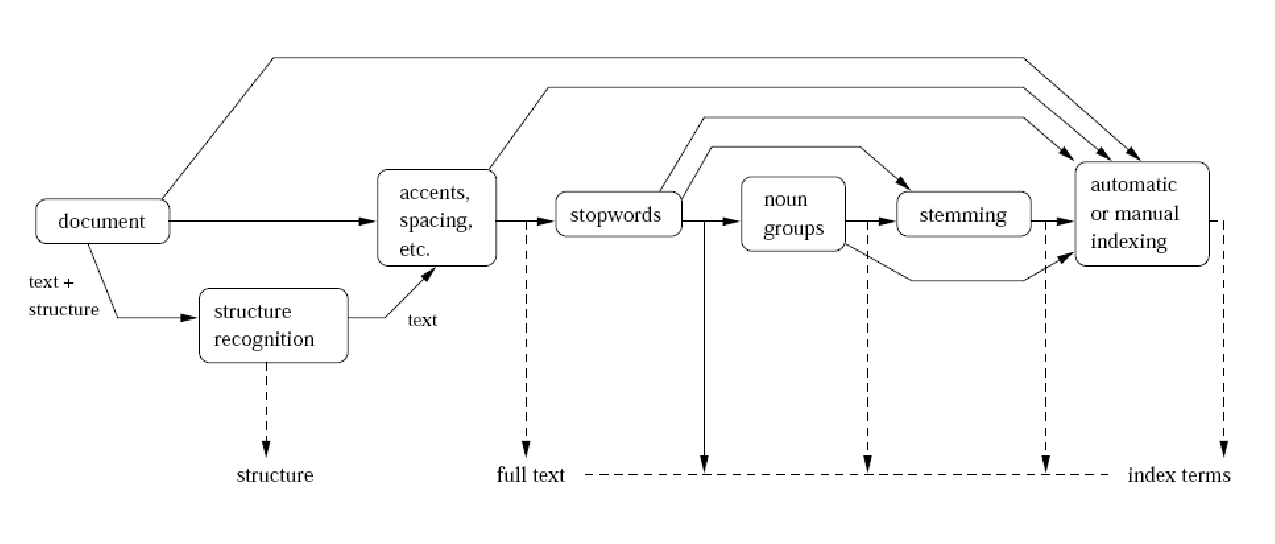
\includegraphics[width=\textwidth]{logical}
  \end{block}  
  
\end{frame}

% ------------------------------------------------------------

%%% usar esta frame com pslatex; ou, em alternativa, a seguinte com pdflatex
%%%
%%% no aquamacs trocar com " ^C ^T ^P	TeX-PDF-mode"

%% \begin{frame}
%%   \begin{center}
%%     \pstree[treesep=1em]{\Mnode[fillcolor=DarkRed]{IR Models}}{
%%       \pstree{\Mnode[fillcolor=Red]{\rnode{BM}{Boolean}}}{
%%         \Mnode[fillcolor=Red]{\rnode{AB}{\shortstack{Fuzzy\\Extended Boolean\\...}}}
%%       }
%%       \pstree{\Mnode[fillcolor=Red]{Vector}}{
%%         \Mnode[fillcolor=Red]{\shortstack{LSI\\Neural Networks\\...}}
%%       }
%%       \pstree{\Mnode[fillcolor=Red]{\rnode{PM}{Probabilistic}}}{
%%         \Mnode[fillcolor=Red]{\shortstack{Belief Network\\Language Models\\...}}
%%       }
%%     }
%%   \end{center}
%%   
%%   \pspolygon[linestyle=dashed,linecolor=Blue,linewidth=0.1mm]([nodesep=-7em,offset=6ex]BM)([nodesep=2em,offset=6ex]PM)([nodesep=2em,offset=-3ex]PM)([nodesep=-7em,offset=-3ex]BM)
%%   \rput[lt]([nodesep=-6.9em,offset=5.5ex]BM){Classic models}
%%   \pspolygon[linestyle=dashed,linecolor=Blue,linewidth=0.1mm]([nodesep=-7em,offset=-5ex]BM)([nodesep=2em,offset=-5ex]PM)([nodesep=2em,offset=-17ex]PM)([nodesep=-7em,offset=-17ex]BM)
%%   \rput[lb]([nodesep=-6.9em,offset=-16.5ex]BM){Alternative models}
%% 
%% 
%% \end{frame}


%% esta frame não funciona com pslatex porque o png n tem BBOX; usar pdflatex

\begin{frame}
  \frametitle{Retrieval Models}

  \begin{center}
    \includegraphics[width=.8\linewidth]{retrieval-models.png}\\
  \end{center}

\end{frame}



\section{Search and The Web}


\begin{frame}
  \frametitle{Motivation for IR Research \& Development}

  \begin{block}{}
    \begin{itemize}
    \item Growing importance of access to information
    \item Growing volume of electronically stored information
    \end{itemize}
  \end{block}

  \begin{center}
    {\Huge $\Downarrow$}
  \end{center}

  \begin{block}{}
    \begin{itemize}
    \item Growing need of efficient and effective means to \emph{organize},
      \emph{store} and \emph{provide access} to information
    \item None of these are trivial tasks
    \end{itemize}
  \end{block}
\end{frame}


\begin{frame}
  \frametitle{How the Web Changed Search}

\begin{block}{Search is everywhere}

\begin{itemize}
\item Web search is today the most prominent application of IR and its
techniques;
\item The ranking and indexing components of any search engine are fundamentally IR pieces of technology. 

\item A \emph{search box} is now common in every web site, app, ...

\end{itemize}
\end{block}

\begin{block}{}
Five major impacts (see next)
\end{block}


\end{frame}


\begin{frame}
  \frametitle{First Major Impact}

The first major impact of the Web on search is related to the \emph{characteristics of the document collection} itself

\begin{itemize}
\item The traditional Web is composed of pages distributed over millions of sites and connected through hyperlinks
\item This requires collecting all documents and storing copies of them in a central repository, prior to indexing
\item This new phase in the IR process, introduced by the Web, is
  called \emph{crawling}
  \begin{itemize}
  \item Many challenges related to the fact that Web contents are very dynamic, and are often hidden behind forms
  \end{itemize}
\end{itemize}

\end{frame}


\begin{frame}
  \frametitle{Second Major Impact}

The second major impact of the Web on search is related to: 
\begin{itemize}
\item The size of the collection
\item The volume of user queries submitted on a daily basis
\end{itemize}

As a consequence, \emph{performance and scalability} have become critical characteristics of IR systems
\vfill
Modern Web-based services (e.g., social media platforms) are further extending the scope of these scalability problems
\end{frame}

\begin{frame}
  \frametitle{Third Major Impact}

In a very large and diverse collection (e.g., documents in multiple languages, of different types, often quite short and ambiguous), \emph{predicting relevance is much harder} than
before
\vfill

Fortunately, the Web also includes new sources of evidence
\begin{itemize} 
  \item hyperlinks 
  \item user clicks in documents in the answer set
  \item complex user profiles
  \item ...
\end{itemize}
\end{frame}


\begin{frame}
  \frametitle{Fourth Major Impact}

The Web is also a medium to do business
\vfill

Search problem has been extended beyond the seeking of text information to also encompass \emph{entities and other user needs}:
\begin{itemize}
  \item the price of a book, 
  \item the phone number of a hotel,
  \item the location of a restaurant,
  \item the link for downloading a software,
  \item ...
\end{itemize}
\vfill
Mobile and voice-based access to the Web has further extended the scope of the problem
\begin{itemize}
\item Increasing importance of \emph{automated assistants} leveraging natural language technologies
\end{itemize}
\end{frame}

\begin{frame}
\frametitle{Fourth Major Impact and Relation to IE}
Advanced search services (e.g., focusing on entities and their properties) often involve \emph{Information Extraction} (IE)
\vfill
Search is made over structured knowledge bases, build through large-scale extraction (e.g., from the Web, e-mails, ...)
\begin{itemize}
\item Knowledge graphs associated to major search engines,
\item Price comparison services,
\item Services like Google Trips,
\item Dialogue services: Siri, Cortana, Alexa, Google Assistant, ...
\end{itemize}
\vfill
Many different Information Extraction challenges:
\begin{itemize}
 \item recognizing and disambiguating entities in text,
 \item extracting properties and relations
 \item ...
\end{itemize}
\end{frame}

\begin{frame}
  \frametitle{Fifth Major Impact}

The fifth major impact of the Web on search is \emph{Web spam}

\begin{block}{Web spam:} 
abusive availability of commercial information disguised in the form of informational content
\end{block}

\vfill

\begin{block}{}
This difficulty is so large that today we even talk of \emph{Adversarial Web Retrieval}.
\end{block}

\end{frame}


\begin{frame}
  \frametitle{Practical Issues in the Web}

\begin{block}{Security}
Commercial transations over the Internet are not yet a completely safe procedure
\end{block}


\begin{block}{Privacy}
 Frequently, people are willing to exchange information as long as it does not become public
\end{block}


\begin{block}{ Copyright and patent rights}
It is far from clear how the widespread data on the Web affects
copyright and patent laws in the various countries
\end{block}

\begin{block}{}
Modern trends relate to multi-modality (e.g., voice interaction through mobile devices) and going beyond {\it search boxes} (e.g., tools that assist in solving complex tasks)
\end{block}

\end{frame}


% ------------------------------------------------------------

\finalframe{Questions?}

\end{document}

%%% Local Variables: 
%%% mode: latex
%%% TeX-master: t
%%% End: 
